\documentclass{article}
\usepackage[french]{babel}
\usepackage[utf8]{inputenc}
\usepackage{graphicx}
\usepackage{dejavu}
\renewcommand*\familydefault{\sfdefault} %% Only if the base font of the document is to be sans serif
\usepackage[T1]{fontenc}

\usepackage{geometry}
\geometry{a4paper,headheight=16pt,tmargin=25mm,
          bmargin=25mm,lmargin=20mm,rmargin=20mm}

\usepackage{fancyhdr}
\usepackage{lastpage}

\usepackage{hyperref}
\usepackage{array}
 
\pagestyle{fancy}
\fancyhf{}
\lhead{\footnotesize Première STI2D\\Tronc commun}
\chead{\large AP Numérisation de l'information : codage binaire}
\lfoot{Lycée Blaise Pascal}
\rfoot{\thepage/\pageref{LastPage}}

\renewcommand{\headrulewidth}{1pt}
\renewcommand{\footrulewidth}{1pt}

\begin{document}
\begin{center}
%	\begin{minipage}[b]{.6\linewidth}
%	\end{minipage}
%	\hfill
%	\begin{minipage}[b]{.3\linewidth}
%		\scriptsize
%		\begin{Form}
%			\TextField[name=nom,width=10em,]{Nom:}\\
%			\TextField[name=prenom,width=10em]{Prénom:}\\
%			\TextField[name=classe,width=10em]{Classe:}\\
%		\end{Form}
%	\end{minipage}
	\begin{flushright}
		\begin{Form}
			\TextField[name=nom,width=10em,default=Nom]{Nom:}\\
			\TextField[name=prenom,width=10em,default=Prénom]{Prénom:}\\
			\TextField[name=classe,width=10em,default=Classe]{Classe:}\\
		\end{Form}
	\end{flushright}

	\vspace{1em}
	\Large
	\textbf{Objectif:} Comment l'ordinateur fait-il pour coder une image?

	\vspace{2em}
	\large
	\textbf{Consigne}: Vous formaliserez vos réponses dans ce document numérique

	\vspace{2em}
	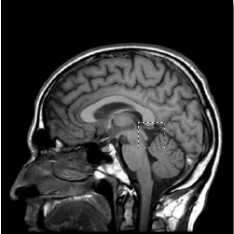
\includegraphics[width=.3\linewidth]{./figures/irm1.png}
	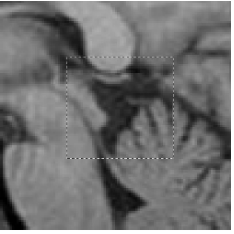
\includegraphics[width=.3\linewidth]{./figures/irm2.png}
	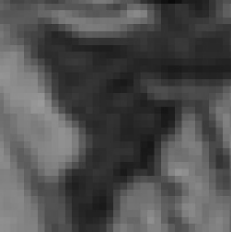
\includegraphics[width=.3\linewidth]{./figures/irm3.png}
\end{center}

\section{Codage d'une image numérique matricielle}
\paragraph{Q1:}
À partir de l'article \href{https://fr.wikipedia.org/wiki/Pixel}{wikipédia sur le pixel}, indiquer:
\begin{itemize}
	\item sa définition;
	\item son abréviation;
	\item la locution anglaise d’où provient le nom \og{}pixel\fg{} ainsi que sa traduction française.
\end{itemize}

\vspace{1em}
\begin{Form}
	\TextField[name=r1,width=\linewidth,height=5em,multiline=true]{}
\end{Form}

\paragraph{Q2:}
Ouvrir le fichier image \og{}stop P5.PGM\fg{} à l'aide du logiciel de visualisation de fichier graphique XNVIEW. 
En zoomant au maximum, indiquer pour l'image considérée:
\begin{itemize}
	\item la largeur (en px);
	\item la hauteur (en px);
	\item le nombre total de pixels.
\end{itemize}

\vspace{1em}
\begin{Form}
	\TextField[name=r2,width=\linewidth,height=5em,multiline=true]{}
\end{Form}

\newpage

\begin{minipage}[b]{.08\linewidth}
	
\includegraphics[width=\linewidth]{./figures/info.png}
\end{minipage}
\hfill
\begin{minipage}[b]{.85\linewidth}
	Pour observer le codage du fichier tel qu’il est dans l’ordinateur, il faut ouvrir l’image avec	un éditeur hexadécimal.
	\vspace{.7em}
\end{minipage}

\paragraph{Q3:}
Tout en laissant ouverte l'image dans Xnview, ouvrir le fichier \og{}stop P5.PGM\fg{}
à l'aide de l’éditeur hexadécimal \og{}Free Hex Editor Neo\fg{} en juxtaposant sur l'écran du PC les 2 représentations (voir ci-dessous).

\begin{center}
	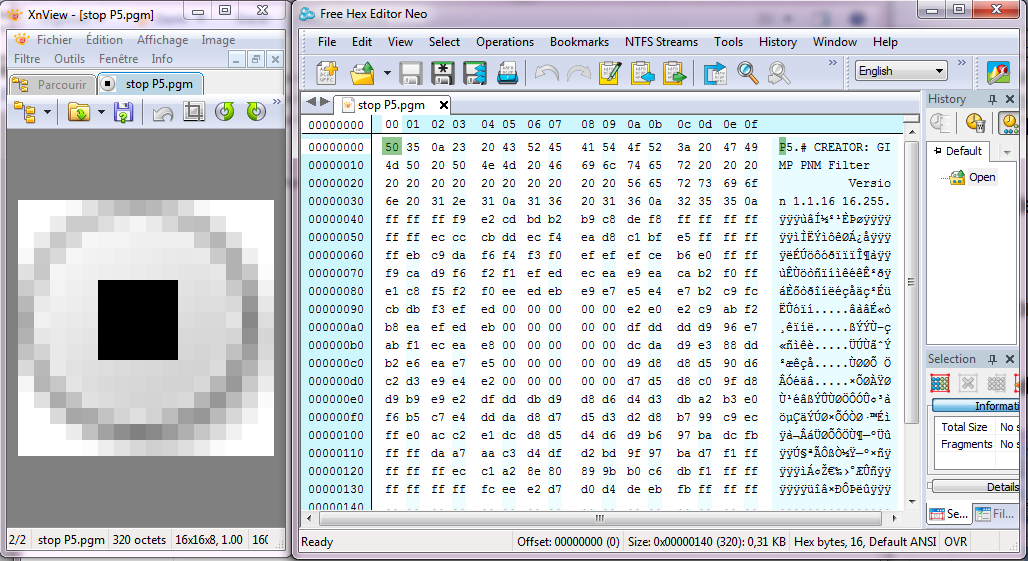
\includegraphics[width=.8\linewidth]{./figures/pic_hex.png}
\end{center}

\paragraph{Q4:}
Dans un premier temps pour faciliter la lecture du fichier dans l'éditeur, on utilisera une représentation en décimal. 
Pour cela, dans l'onglet \og{}View\fg{} spécifier \og{}decimal\fg{} pour les réglages \og{}Offset\fg{} et \og{}Display As\fg{} (voir ci-dessous).

\begin{center}
	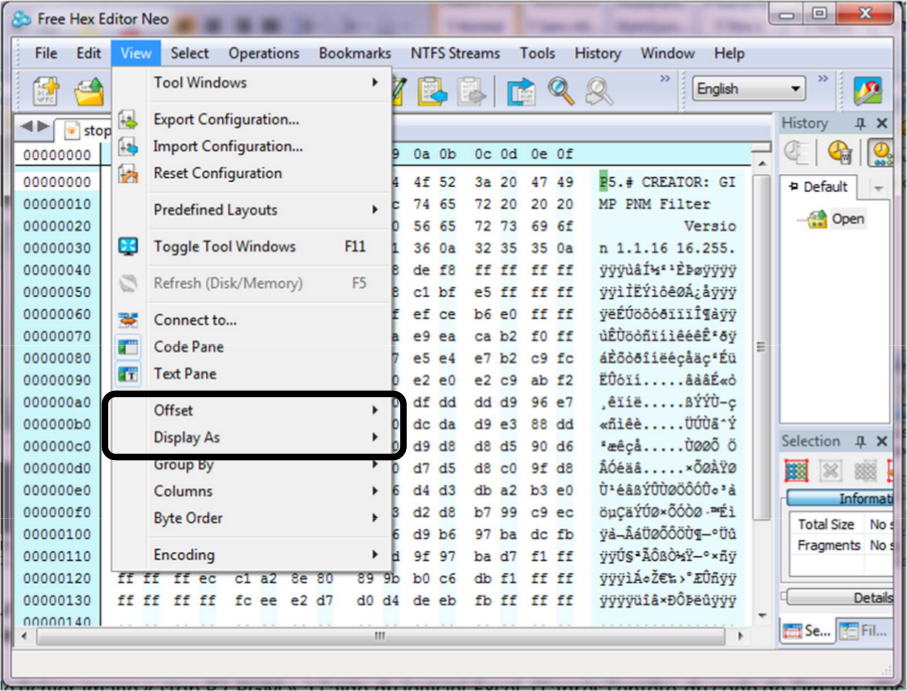
\includegraphics[width=.6\linewidth]{./figures/config_decimal.png}
\end{center}

\begin{center}
	\vspace{2em}
	\Large
	\textbf{Faire valider par l'enseignant}
\end{center}

\newpage

\paragraph{Q5:}
À partir de l'article \href{https://fr.wikipedia.org/wiki/Header}{wikipédia de l'entête d’un fichier}, indiquer dans le cas d'une image:
\begin{itemize}
	\item les informations pouvant être contenues dans l'entête;
	\item la traduction anglaise de \og{}entête\fg{}.
\end{itemize}

\vspace{1em}
\begin{Form}
	\TextField[name=r5,width=\linewidth,height=5em,multiline=true]{}
\end{Form}

Dans l'éditeur hexadécimal, on retrouve la zone du fichier correspondant à l'entête et celle correspondant à l'image.\\

De plus la représentation du codage s’effectue sous deux formes:
\begin{itemize}
	\item À gauche on visualise le codage au format décimal (qui apparaît comme des cases);
	\item À droite la correspondance au format texte.\\
\end{itemize}

Enfin la colonne de gauche, permet de déterminer le numéro de la case du fichier.\\

\begin{center}
	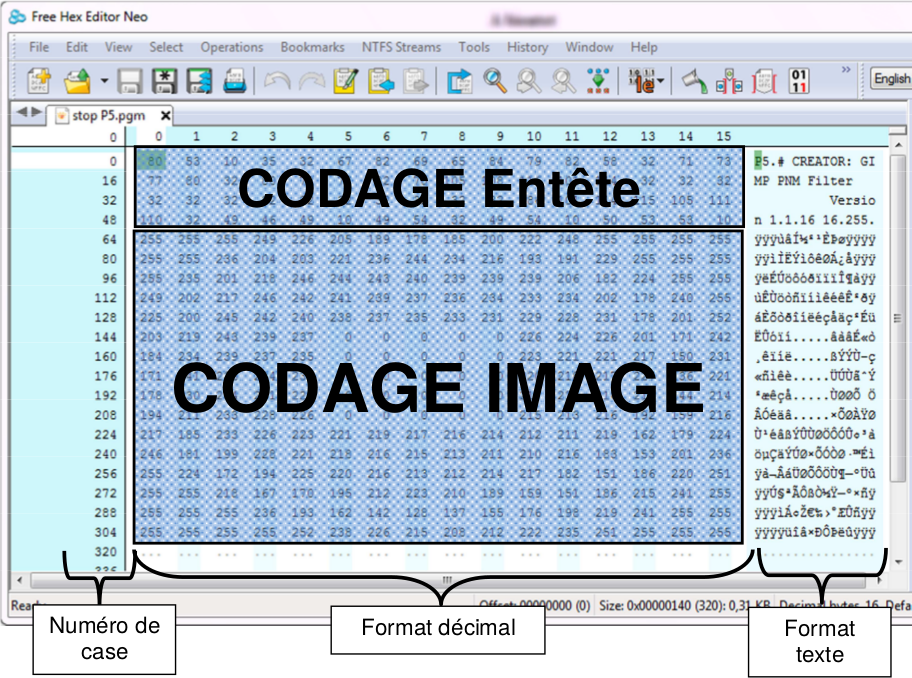
\includegraphics[width=.8\linewidth]{./figures/header_hex.png}
\end{center}

\paragraph{Q6:}
Dans la zone de l'entête codé en format texte, retrouvez la hauteur et la largeur de l'image.

\vspace{1em}
\begin{Form}
	\TextField[name=r6,width=\linewidth,height=5em,multiline=true]{}
\end{Form}

\newpage

\paragraph{Q7:}
Toujours dans la zone de l'entête codé en format texte, 
le premier nombre qui suit la hauteur et la largeur de l'image indique le nombre maximal de niveaux de gris pouvant être représentés dans l'image.\\

Combien peut-il exister de niveaux de gris différents dans cette image ?

\vspace{1em}
\begin{Form}
	\TextField[name=r7,width=\linewidth,height=5em,multiline=true]{}
\end{Form}

\paragraph{Q8:}
Toujours en juxtaposant sur l'écran du PC le fichier \og{}stop P5.PGM\fg{} ouvert à la fois dans \og{}XNVIEW\fg{} et dans \og{}Free Hex Editor Neo\fg{}, 
modifier judicieusement quelques valeurs de pixels dans \og{}Free Hex Editor Neo\fg{} et observer la modification de l'image 
(penser à raffraîchir l'image dans \og{}XNVIEW\fg{} avec CTRL+R) de façon à répondre aux questions suivantes:
\begin{itemize}
	\item Quel nombre est utilisé pour coder le blanc ?
	\item Quel nombre est utilisé pour coder le noir ?
	\item À quoi correspondent les nombres compris entre 1 et 254 ?
\end{itemize}

\vspace{1em}
\begin{Form}
	\TextField[name=r8,width=\linewidth,height=5em,multiline=true]{}
\end{Form}

\begin{minipage}[b]{.8\linewidth}
	\paragraph{Q9:}
	Modifier les valeurs du fichier \og{}stop P5.PGM\fg{} de façon à obtenir l'image ci-contre dans \og{}Xnview\fg{}.
	\vspace{2em}
\end{minipage}
\hfill
\begin{minipage}[b]{.12\linewidth}
	
\includegraphics[width=\linewidth]{./figures/stop_modif.png}
\end{minipage}

\begin{center}
	\Large
	\textbf{Faire valider par l'enseignant}
\end{center}

\paragraph{Q10:}
À l'aide de la colonne de gauche de \og{}Free Hex Editor Neo\fg{}, déterminer le nombre total de cases permettant de coder la totalité du fichier, 
soit l'entête et l'image.

\vspace{1em}
\begin{Form}
	\TextField[name=r10,width=\linewidth,height=5em,multiline=true]{}
\end{Form}

\paragraph{Q11:}
Sous l'explorateur windows, en exploitant les propriétés du fichier \og{}stop P5.PGM\fg{}, indiquer sa taille réelle. 
En déduire ce que représente une case du fichier.

\vspace{1em}
\begin{Form}
	\TextField[name=r11,width=\linewidth,height=5em,multiline=true]{}
\end{Form}

\newpage

\paragraph{Q12:}
À partir d'une recherche internet, donner la définition d'un octet.

\vspace{1em}
\begin{Form}
	\TextField[name=r12,width=\linewidth,height=5em,multiline=true]{}
\end{Form}

\paragraph{Q13:}
Dans \og{}Free Hex Editor Neo\fg{}, modifier les valeurs de la ligne supérieure de l'image de façon à avoir la suite des nombres de 0 à 15 (voir ci-dessous).

\begin{center}
	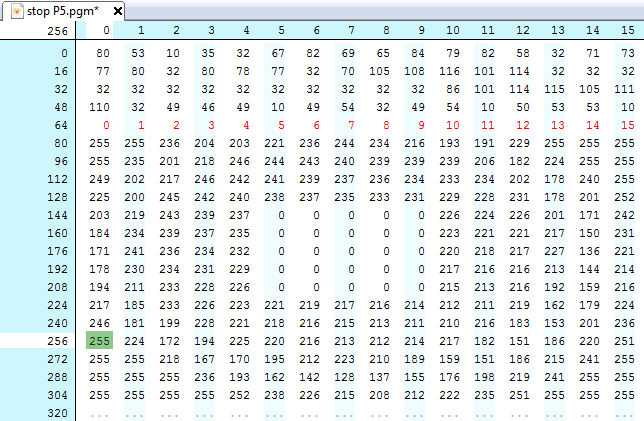
\includegraphics[width=.8\linewidth]{./figures/hex_0to15.png}
\end{center}

\begin{center}
	\Large
	\textbf{Faire valider par l'enseignant}
\end{center}

\paragraph{Q14:}
Dans \og{}Free Hex Editor Neo\fg{}, 
changer la base de représentation des nombres de décimal à binaire en cliquant sur l'onglet \og{}View\fg{} puis \og{}displays as\fg{} puis \og{}binary\fg{}. 
En déduire combien d'informations binaires contient une case.
 
\vspace{1em}
\begin{Form}
	\TextField[name=r14,width=\linewidth,height=5em,multiline=true]{}
\end{Form}

\newpage

\paragraph{Q15:}
Compléter le tableau ci-dessous.

\vspace{1em}
\begin{Form}
	\begin{tabular}{|>{\centering\arraybackslash}m{8em}||c|c|c|c|c|c|c|c|}
	\hline
	Représentation décimale & \multicolumn{8}{c|}{Représentation binaire} \\
	\hline
	\hline
	0 & \TextField[name=b00,width=3em]{} & \TextField[name=b01,width=3em]{} & \TextField[name=b02,width=3em]{} & \TextField[name=b03,width=3em]{} & \TextField[name=b04,width=3em] & {}\TextField[name=b05,width=3em]{} & \TextField[name=b06,width=3em]{} & \TextField[name=b07,width=3em]{} \\
	\hline
	1 & \TextField[name=b10,width=3em]{} & \TextField[name=b11,width=3em]{} & \TextField[name=b12,width=3em]{} & \TextField[name=b13,width=3em]{} & \TextField[name=b14,width=3em] & {}\TextField[name=b15,width=3em]{} & \TextField[name=b16,width=3em]{} & \TextField[name=b17,width=3em]{} \\
	\hline
	2 & \TextField[name=b20,width=3em]{} & \TextField[name=b21,width=3em]{} & \TextField[name=b22,width=3em]{} & \TextField[name=b23,width=3em]{} & \TextField[name=b24,width=3em] & {}\TextField[name=b25,width=3em]{} & \TextField[name=b26,width=3em]{} & \TextField[name=b27,width=3em]{} \\
	\hline
	3 & \TextField[name=b30,width=3em]{} & \TextField[name=b31,width=3em]{} & \TextField[name=b32,width=3em]{} & \TextField[name=b33,width=3em]{} & \TextField[name=b34,width=3em] & {}\TextField[name=b35,width=3em]{} & \TextField[name=b36,width=3em]{} & \TextField[name=b37,width=3em]{} \\
	\hline
	4 & \TextField[name=b40,width=3em]{} & \TextField[name=b41,width=3em]{} & \TextField[name=b42,width=3em]{} & \TextField[name=b43,width=3em]{} & \TextField[name=b44,width=3em] & {}\TextField[name=b45,width=3em]{} & \TextField[name=b46,width=3em]{} & \TextField[name=b47,width=3em]{} \\
	\hline
	5 & \TextField[name=b50,width=3em]{} & \TextField[name=b51,width=3em]{} & \TextField[name=b52,width=3em]{} & \TextField[name=b53,width=3em]{} & \TextField[name=b54,width=3em] & {}\TextField[name=b55,width=3em]{} & \TextField[name=b56,width=3em]{} & \TextField[name=b57,width=3em]{} \\
	\hline
	6 & \TextField[name=b60,width=3em]{} & \TextField[name=b61,width=3em]{} & \TextField[name=b62,width=3em]{} & \TextField[name=b63,width=3em]{} & \TextField[name=b64,width=3em] & {}\TextField[name=b65,width=3em]{} & \TextField[name=b66,width=3em]{} & \TextField[name=b67,width=3em]{} \\
	\hline
	7 & \TextField[name=b70,width=3em]{} & \TextField[name=b71,width=3em]{} & \TextField[name=b72,width=3em]{} & \TextField[name=b73,width=3em]{} & \TextField[name=b74,width=3em] & {}\TextField[name=b75,width=3em]{} & \TextField[name=b76,width=3em]{} & \TextField[name=b77,width=3em]{} \\
	\hline
	8 & \TextField[name=b80,width=3em]{} & \TextField[name=b81,width=3em]{} & \TextField[name=b82,width=3em]{} & \TextField[name=b83,width=3em]{} & \TextField[name=b84,width=3em] & {}\TextField[name=b85,width=3em]{} & \TextField[name=b86,width=3em]{} & \TextField[name=b87,width=3em]{} \\
	\hline
	9 & \TextField[name=b90,width=3em]{} & \TextField[name=b91,width=3em]{} & \TextField[name=b92,width=3em]{} & \TextField[name=b93,width=3em]{} & \TextField[name=b94,width=3em] & {}\TextField[name=b95,width=3em]{} & \TextField[name=b96,width=3em]{} & \TextField[name=b97,width=3em]{} \\
	\hline
	10 & \TextField[name=ba0,width=3em]{} & \TextField[name=ba1,width=3em]{} & \TextField[name=ba2,width=3em]{} & \TextField[name=ba3,width=3em]{} & \TextField[name=ba4,width=3em] & {}\TextField[name=ba5,width=3em]{} & \TextField[name=ba6,width=3em]{} & \TextField[name=ba7,width=3em]{} \\
	\hline
	11 & \TextField[name=bbc,width=3em]{} & \TextField[name=bb1,width=3em]{} & \TextField[name=bb2,width=3em]{} & \TextField[name=bb3,width=3em]{} & \TextField[name=bb4,width=3em] & {}\TextField[name=bb5,width=3em]{} & \TextField[name=bb6,width=3em]{} & \TextField[name=bb7,width=3em]{} \\
	\hline
	12 & \TextField[name=bc0,width=3em]{} & \TextField[name=bc1,width=3em]{} & \TextField[name=bc2,width=3em]{} & \TextField[name=bc3,width=3em]{} & \TextField[name=bc4,width=3em] & {}\TextField[name=bc5,width=3em]{} & \TextField[name=bc6,width=3em]{} & \TextField[name=bc7,width=3em]{} \\
	\hline
	13 & \TextField[name=bd0,width=3em]{} & \TextField[name=bd1,width=3em]{} & \TextField[name=bd2,width=3em]{} & \TextField[name=bd3,width=3em]{} & \TextField[name=bd4,width=3em] & {}\TextField[name=bd5,width=3em]{} & \TextField[name=bd6,width=3em]{} & \TextField[name=bd7,width=3em]{} \\
	\hline
	14 & \TextField[name=be0,width=3em]{} & \TextField[name=be1,width=3em]{} & \TextField[name=be2,width=3em]{} & \TextField[name=be3,width=3em]{} & \TextField[name=be4,width=3em] & {}\TextField[name=be5,width=3em]{} & \TextField[name=be6,width=3em]{} & \TextField[name=be7,width=3em]{} \\
	\hline
	15 & \TextField[name=bf0,width=3em]{} & \TextField[name=bf1,width=3em]{} & \TextField[name=bf2,width=3em]{} & \TextField[name=bf3,width=3em]{} & \TextField[name=bf4,width=3em] & {}\TextField[name=bf5,width=3em]{} & \TextField[name=bf6,width=3em]{} & \TextField[name=bf7,width=3em]{} \\
	\hline
\end{tabular}
\end{Form}

\paragraph{Q16:}
En faisant l'opération inverse dans \og{}Free Hex Editor Neo\fg{}, convertir les nombres binaires ci-dessous en décimal.

\vspace{1em}
\begin{center}
	\begin{Form}
		\begin{tabular}{|>{\centering\arraybackslash}m{8em}||c|c|c|c|c|c|c|c|}
			\hline
			Représentation décimale & \multicolumn{8}{c|}{Représentation binaire} \\
			\hline
			\hline
			\TextField[name=d0,width=6em]{} & 0 & 0 & 0 & 0 & 0 & 0 & 0 & 0\\
			\hline
			\TextField[name=d1,width=6em]{} & 0 & 0 & 0 & 0 & 0 & 0 & 0 & 1\\
			\hline
			\TextField[name=d2,width=6em]{} & 0 & 0 & 0 & 0 & 0 & 0 & 1 & 0\\
			\hline
			\TextField[name=d3,width=6em]{} & 0 & 0 & 0 & 0 & 0 & 1 & 0 & 0\\
			\hline
			\TextField[name=d4,width=6em]{} & 0 & 0 & 0 & 0 & 1 & 0 & 0 & 0\\
			\hline
			\TextField[name=d5,width=6em]{} & 0 & 0 & 0 & 1 & 0 & 0 & 0 & 0\\
			\hline
			\TextField[name=d6,width=6em]{} & 0 & 0 & 1 & 0 & 0 & 0 & 0 & 0\\
			\hline
			\TextField[name=d7,width=6em]{} & 0 & 1 & 0 & 0 & 0 & 0 & 0 & 0\\
			\hline
			\TextField[name=d8,width=6em]{} & 1 & 0 & 0 & 0 & 0 & 0 & 0 & 0\\
			\hline
			\TextField[name=d9,width=6em]{} & 1 & 1 & 1 & 1 & 1 & 1 & 1 & 1\\
			\hline
		\end{tabular}
	\end{Form}
\end{center}

\newpage

\begin{minipage}[b]{.08\linewidth}
	
\includegraphics[width=\linewidth]{./figures/info.png}
	\vspace{1em}
\end{minipage}
\hfill
\begin{minipage}[b]{.85\linewidth}
	Pour passer de la représentation binaire à la représentation décimale, 
	on peut s'aider d'un tableau de deux lignes.

	La première ligne contient les \textbf{bits du nombre à convertir}. La deuxième ligne quant à elle contient la \textbf{liste des puissances de deux} croissantes de droite à gauche.

	Pour chaque colonne, on multiplie le contenu des deux lignes, puis on additionne le résultat de chaque multiplication.
\end{minipage}

\paragraph{Exemple:} 
Si l'on veut convertir le nombre représenté en binaire $N_{binaire} =$ \texttt{0100 0100} en décimal, on remplit le tableau de la manière suivante:

\begin{center}
	\begin{tabular}{|c|c|c|c|c|c|c|c|}
		\hline
		0 & 1 & 0 & 0 & 0 & 1 & 0 & 0 \\
		\hline
		$2^7 = 128$ & $2^6 = 64$ & $2^5 = 32$ & $2^4 = 16$ & $2^3 = 8$ & $2^2 = 4$ & $2^1 = 2$ & $2^0 = 1$ \\
		\hline
	\end{tabular}
\end{center}

On peut maintenant calculer la représentation décimale de notre nombre :
$$N_{decimal} = 1 \times 2^6 + 1 \times 2^2 = 1 \times 64 + 1 \times 4 = 68$$
\paragraph{Q17:}
Entrez votre date de naissance 
\begin{Form}
	\TextField[name=jj,width=2em,default=jj]{} / \TextField[name=mm,width=2em,default=mm]{} / \TextField[name=aa,width=2em,default=aa]{}\\
\end{Form}

À l'aide du tableau ci-dessous, convertir vos jour, mois et année de naissance en binaire.

\begin{center}
	\begin{tabular}{|r||c|c|c|c|c|c|c|c|}
		\hline
		Jour & \TextField[name=jj0,width=3em]{} & \TextField[name=jj1,width=3em]{} & \TextField[name=jj2,width=3em]{} & \TextField[name=jj3,width=3em]{} & \TextField[name=jj4,width=3em] & {}\TextField[name=jj5,width=3em]{} & \TextField[name=jj6,width=3em]{} & \TextField[name=jj7,width=3em]{} \\
		\hline
		Mois & \TextField[name=mm0,width=3em]{} & \TextField[name=mm1,width=3em]{} & \TextField[name=mm2,width=3em]{} & \TextField[name=mm3,width=3em]{} & \TextField[name=mm4,width=3em] & {}\TextField[name=mm5,width=3em]{} & \TextField[name=mm6,width=3em]{} & \TextField[name=mm7,width=3em]{} \\
		\hline
		Année & \TextField[name=aa0,width=3em]{} & \TextField[name=aa1,width=3em]{} & \TextField[name=aa2,width=3em]{} & \TextField[name=aa3,width=3em]{} & \TextField[name=aa4,width=3em] & {}\TextField[name=aa5,width=3em]{} & \TextField[name=aa6,width=3em]{} & \TextField[name=aa7,width=3em]{} \\
		\hline
		\hline
		& 128 & 64 & 32 & 16 & 8 & 4 & 2 & 1 \\
		\hline
	\end{tabular}
\end{center}

\newpage

\paragraph{Q18:}
Lire cet article \href{http://www.semageek.com/bbc-horloge-binaire-gante/}{http://www.semageek.com/bbc-horloge-binaire-gante/} puis répondre aux questions suivantes:\\

Retrouver l’heure correspondante aux 4 affichages de l’horloge binaire:

\vspace{2em}

\begin{minipage}[b]{.3\linewidth}
	\begin{Form}
		\begin{center}
			\TextField[name=bbc1h,width=2em]{}h \TextField[name=bbc1m,width=2em]{}min \TextField[name=bbc1s,width=2em]{}s
			\vspace{2em}
		\end{center}
	\end{Form}
\end{minipage}
\hfill
\begin{minipage}[b]{.6\linewidth}
	\centering
	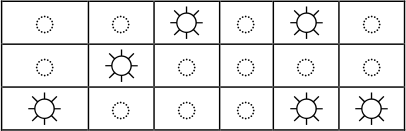
\includegraphics[width=.7\linewidth]{./figures/bbc1.png}
\end{minipage}

\vspace{2em}

\begin{minipage}[b]{.3\linewidth}
	\begin{Form}
		\begin{center}
			\TextField[name=bbc2h,width=2em]{}h \TextField[name=bbc2m,width=2em]{}min \TextField[name=bbc2s,width=2em]{}s
			\vspace{2em}
		\end{center}
	\end{Form}
\end{minipage}
\hfill
\begin{minipage}[b]{.6\linewidth}
	\centering
	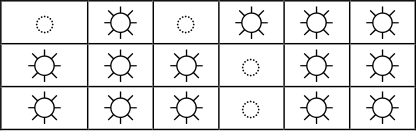
\includegraphics[width=.7\linewidth]{./figures/bbc2.png}
\end{minipage}

\vspace{2em}

\begin{minipage}[b]{.3\linewidth}
	\begin{Form}
		\begin{center}
			\TextField[name=bbc3h,width=2em]{}h \TextField[name=bbc3m,width=2em]{}min \TextField[name=bbc3s,width=2em]{}s
			\vspace{2em}
		\end{center}
	\end{Form}
\end{minipage}
\hfill
\begin{minipage}[b]{.6\linewidth}
	\centering
	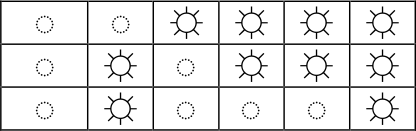
\includegraphics[width=.7\linewidth]{./figures/bbc3.png}
\end{minipage}

\vspace{2em}

\begin{minipage}[b]{.3\linewidth}
	\begin{Form}
		\begin{center}
			\TextField[name=bbc4h,width=2em]{}h \TextField[name=bbc4m,width=2em]{}min \TextField[name=bbc4s,width=2em]{}s
			\vspace{2em}
		\end{center}
	\end{Form}
\end{minipage}
\hfill
\begin{minipage}[b]{.6\linewidth}
	\centering
	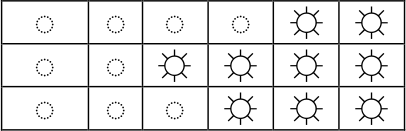
\includegraphics[width=.7\linewidth]{./figures/bbc4.png}
\end{minipage}

\vspace{2em}

Indiquer les cercles de LED à éclairer de façon à coder en binaire les 4 heures ci-dessous:

\vspace{2em}

\begin{minipage}[b]{.3\linewidth}
	\begin{Form}
		\begin{center}
			8h 5min 45s
			\vspace{.4em}
		\end{center}
	\end{Form}
\end{minipage}
\hfill
\begin{minipage}[b]{.6\linewidth}
	\begin{center}
		\begin{Form}
			\begin{tabular}{|c|c|c|c|c|c|}
				\hline
%				\CheckBox[name=bbch5,width=1em]{} & \CheckBox[name=bbch4,width=1em]{} & \CheckBox[name=bbch3,width=1em]{} & \CheckBox[name=bbch2,width=1em]{} & \CheckBox[name=bbch1,width=1em]{} & \CheckBox[name=bbch0,width=1em]{}\\
				\TextField[name=bbc1h5,width=2em]{} & \TextField[name=bbc1h4,width=2em]{} & \TextField[name=bbc1h3,width=2em]{} & \TextField[name=bbc1h2,width=2em]{} & \TextField[name=bbc1h1,width=2em]{} & \TextField[name=bbc1h0,width=2em]{}\\
				\hline
				\TextField[name=bbc1m5,width=2em]{} & \TextField[name=bbc1m4,width=2em]{} & \TextField[name=bbc1m3,width=2em]{} & \TextField[name=bbc1m2,width=2em]{} & \TextField[name=bbc1m1,width=2em]{} & \TextField[name=bbc1m0,width=2em]{}\\
				\hline
				\TextField[name=bbc1s5,width=2em]{} & \TextField[name=bbc1s4,width=2em]{} & \TextField[name=bbc1s3,width=2em]{} & \TextField[name=bbc1s2,width=2em]{} & \TextField[name=bbc1s1,width=2em]{} & \TextField[name=bbc1s0,width=2em]{}\\
				\hline
			\end{tabular}
		\end{Form}
	\end{center}
\end{minipage}

\vspace{2em}

\begin{minipage}[b]{.3\linewidth}
	\begin{Form}
		\begin{center}
			19h 20min 37s
			\vspace{.4em}
		\end{center}
	\end{Form}
\end{minipage}
\hfill
\begin{minipage}[b]{.6\linewidth}
	\begin{center}
		\begin{Form}
			\begin{tabular}{|c|c|c|c|c|c|}
				\hline
%				\CheckBox[name=bbch5,width=1em]{} & \CheckBox[name=bbch4,width=1em]{} & \CheckBox[name=bbch3,width=1em]{} & \CheckBox[name=bbch2,width=1em]{} & \CheckBox[name=bbch1,width=1em]{} & \CheckBox[name=bbch0,width=1em]{}\\
				\TextField[name=bbc2h5,width=2em]{} & \TextField[name=bbc2h4,width=2em]{} & \TextField[name=bbc2h3,width=2em]{} & \TextField[name=bbc2h2,width=2em]{} & \TextField[name=bbc2h1,width=2em]{} & \TextField[name=bbc2h0,width=2em]{}\\
				\hline
				\TextField[name=bbc2m5,width=2em]{} & \TextField[name=bbc2m4,width=2em]{} & \TextField[name=bbc2m3,width=2em]{} & \TextField[name=bbc2m2,width=2em]{} & \TextField[name=bbc2m1,width=2em]{} & \TextField[name=bbc2m0,width=2em]{}\\
				\hline
				\TextField[name=bbc2s5,width=2em]{} & \TextField[name=bbc2s4,width=2em]{} & \TextField[name=bbc2s3,width=2em]{} & \TextField[name=bbc2s2,width=2em]{} & \TextField[name=bbc2s1,width=2em]{} & \TextField[name=bbc2s0,width=2em]{}\\
				\hline
			\end{tabular}
		\end{Form}
	\end{center}
\end{minipage}

\vspace{2em}

\begin{minipage}[b]{.3\linewidth}
	\begin{Form}
		\begin{center}
			12h 50min 23s
			\vspace{.4em}
		\end{center}
	\end{Form}
\end{minipage}
\hfill
\begin{minipage}[b]{.6\linewidth}
	\begin{center}
		\begin{Form}
			\begin{tabular}{|c|c|c|c|c|c|}
				\hline
%				\CheckBox[name=bbch5,width=1em]{} & \CheckBox[name=bbch4,width=1em]{} & \CheckBox[name=bbch3,width=1em]{} & \CheckBox[name=bbch2,width=1em]{} & \CheckBox[name=bbch1,width=1em]{} & \CheckBox[name=bbch0,width=1em]{}\\
				\TextField[name=bbc3h5,width=2em]{} & \TextField[name=bbc3h4,width=2em]{} & \TextField[name=bbc3h3,width=2em]{} & \TextField[name=bbc3h2,width=2em]{} & \TextField[name=bbc3h1,width=2em]{} & \TextField[name=bbc3h0,width=2em]{}\\
				\hline
				\TextField[name=bbc3m5,width=2em]{} & \TextField[name=bbc3m4,width=2em]{} & \TextField[name=bbc3m3,width=2em]{} & \TextField[name=bbc3m2,width=2em]{} & \TextField[name=bbc3m1,width=2em]{} & \TextField[name=bbc3m0,width=2em]{}\\
				\hline
				\TextField[name=bbc3s5,width=2em]{} & \TextField[name=bbc3s4,width=2em]{} & \TextField[name=bbc3s3,width=2em]{} & \TextField[name=bbc3s2,width=2em]{} & \TextField[name=bbc3s1,width=2em]{} & \TextField[name=bbc3s0,width=2em]{}\\
				\hline
			\end{tabular}
		\end{Form}
	\end{center}
\end{minipage}

\vspace{2em}

\begin{minipage}[b]{.3\linewidth}
	\begin{Form}
		\begin{center}
			21h 31min 57s
			\vspace{.4em}
		\end{center}
	\end{Form}
\end{minipage}
\hfill
\begin{minipage}[b]{.6\linewidth}
	\begin{center}
		\begin{Form}
			\begin{tabular}{|c|c|c|c|c|c|}
				\hline
%				\CheckBox[name=bbch5,width=1em]{} & \CheckBox[name=bbch4,width=1em]{} & \CheckBox[name=bbch3,width=1em]{} & \CheckBox[name=bbch2,width=1em]{} & \CheckBox[name=bbch1,width=1em]{} & \CheckBox[name=bbch0,width=1em]{}\\
				\TextField[name=bbc4h5,width=2em]{} & \TextField[name=bbc4h4,width=2em]{} & \TextField[name=bbc4h3,width=2em]{} & \TextField[name=bbc4h2,width=2em]{} & \TextField[name=bbc4h1,width=2em]{} & \TextField[name=bbc4h0,width=2em]{}\\
				\hline
				\TextField[name=bbc4m5,width=2em]{} & \TextField[name=bbc4m4,width=2em]{} & \TextField[name=bbc4m3,width=2em]{} & \TextField[name=bbc4m2,width=2em]{} & \TextField[name=bbc4m1,width=2em]{} & \TextField[name=bbc4m0,width=2em]{}\\
				\hline
				\TextField[name=bbc4s5,width=2em]{} & \TextField[name=bbc4s4,width=2em]{} & \TextField[name=bbc4s3,width=2em]{} & \TextField[name=bbc4s2,width=2em]{} & \TextField[name=bbc4s1,width=2em]{} & \TextField[name=bbc4s0,width=2em]{}\\
				\hline
			\end{tabular}
		\end{Form}
	\end{center}
\end{minipage}
\end{document}
